%%%%%%%%%%%%%%%%%%%%%%%%%%%%%%%%%%%%%%%%%%%%%%%%%%%%%%%%%%%%%%
%% Rozdział 4: Rozpoznawanie izolowanych glos (video2gloss)
%%%%%%%%%%%%%%%%%%%%%%%%%%%%%%%%%%%%%%%%%%%%%%%%%%%%%%%%%%%%%%

\section{Rozpoznawanie izolowanych glos (video2gloss)}
\label{chap:isolated-gloss-recognition}

W celu realizacji zadania przekształcania obrazu wideo na glosę, wprowadzonego w
Rozdziale~\ref{chap:related-work}, przyjmujemy podejście oparte na wyszukiwaniu:
zamiast uczyć model stałego zbioru granic klas, uczymy przestrzeń osadzeń, w której
przykłady tej samej glosy tworzą skupiska, a klasyfikację pozostawiamy etapowi
wyszukiwania najbliższych sąsiadów w tej przestrzeni
(Rysunek~\ref{fig:slt-problem-overview}). Takie sformułowanie lepiej radzi sobie
ze zmiennością wewnątrzklasową niż klasyfikator softmax, naturalnie skaluje się
do nowego słownictwa bez konieczności ponownego trenowania głowicy
klasyfikacyjnej oraz zapewnia bazę reprezentacyjną odpowiednią do rozszerzeń
opartych na dopasowaniu i rozpoznawania ciągłego, omówionych w
Sekcji~\ref{sec:gloss-recognition-discussion}.

\begin{figure}[htbp]
  \centering
  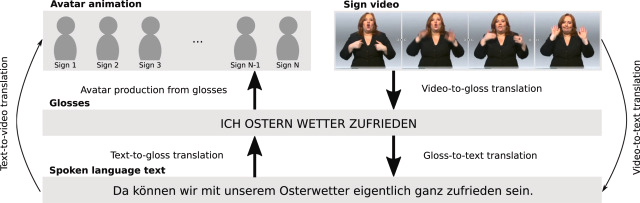
\includegraphics[width=0.85\textwidth]{figures/gloss-recognition/slt-problem-overview.png}
  \caption{Ogólny problem tłumaczenia języka migowego oraz pozycja zadania
  przekształcania obrazu wideo na glosę w ramach tego problemu.}
  \label{fig:slt-problem-overview}
\end{figure}

Wkład niniejszego rozdziału obejmuje: (i) sformułowanie rozpoznawania izolowanych
glos z obrazu wideo jako problemu opartego na wyszukiwaniu, w którym rozpoznawanie
glos jest realizowane poprzez uczenie metryczne, a następnie wyszukiwanie
najbliższych sąsiadów; (ii) wielokryterialny schemat treningowy łączący funkcję
straty Multi-Similarity dla uczenia metrycznego z pomocniczym celem rekonstrukcji
punktów charakterystycznych; (iii) kontrolowany benchmark pięciu enkoderów
czasowych -- Transformer, LSTM, BiLSTM, GRU i BiGRU -- przy identycznym
przetwarzaniu wstępnym, próbkowaniu, funkcji straty i konfiguracji treningowej;
oraz (iv) geometryczną charakterystykę problemu zmienności między osobami
migającymi poprzez analizę macierzy pomyłek, czułości dla poszczególnych klas,
wizualizację t-SNE oraz śledzenie odległości par pozytywnych i negatywnych.

\subsection{Zbiór danych i przetwarzanie wstępne}
\label{sec:gloss-recognition-dataset}

Eksperymenty przedstawione w tym rozdziale przeprowadzono na podzbiorze zbioru
danych ASL Citizen (Microsoft, 2023), wielkoskalowego korpusu amerykańskiego
języka migowego, zebranego z naciskiem na różnorodność osób migających oraz
wiarygodność warunków rzeczywistych. Pełny zbiór danych obejmuje 1{,}068
opatrzonych adnotacjami nagrań migania, obejmujących szeroki zakres leksykalny.
Na potrzeby benchmarku wybrano podzbiór 32 glos, reprezentujących różnorodne
kategorie semantyczne -- przedmioty codziennego użytku, czynności, określenia
czasowe, kolory oraz role społeczne:

\begin{quote}
\small
BASKETBALL, BEE, BREAKFAST, CALL, CAR, CAT, CHRISTMAS, DEAF, DOG, EAT, FIREMAN,
FISH, FOOTBALL, GREEN, HEAD, HOSPITAL, KID, LUNCH, MAN, MECHANIC, MORNING,
NIGHT, NO, NOON, RED, SMILE, STUDENT, TRIP, UNIVERSITY, VALUE, WOMAN, YES.
\end{quote}

\label{sec:gloss-recognition-preprocessing}
Proces przetwarzania wstępnego nie operuje na surowym obrazie wideo, lecz na
sekwencjach punktów charakterystycznych dla kolejnych klatek, wyodrębnionych za
pomocą MediaPipe i wygenerowanych przez platformę adnotacyjną opisaną w
Sekcji~\ref{sec:annotation-data-format}. Każda klatka jest reprezentowana przez
wektor o 144 wymiarach, obejmujący wybrany podzbiór punktów charakterystycznych
pozy górnej części ciała oraz pełne zbiory punktów charakterystycznych lewej i
prawej dłoni. MediaPipe działa na poziomie pojedynczej klatki, generując
współrzędne dla zestawu anatomicznie zdefiniowanych punktów ciała -- w tym
stawów takich jak nadgarstki, kostki dłoni i końcówki palców -- przy czym każdy
punkt jest opisywany jako pozycja 3D względem określonego anatomicznego punktu
odniesienia: środka bioder dla pozy ciała oraz nadgarstka dla punktów dłoni
(Rysunek~\ref{fig:mediapipe-intuition} i
Rysunek~\ref{fig:mediapipe-holistic-landmarks}). Operowanie na sekwencjach
punktów charakterystycznych zamiast na surowych klatkach wideo sprzyja
generalizacji pomiędzy osobami migającymi poprzez abstrahowanie od zmienności
na poziomie wyglądu, takiej jak odcień skóry, ubiór czy oświetlenie, oraz kieruje
uwagę modelu na sygnał najbardziej istotny dla języka migowego: uporządkowany
ruch ludzkiego ciała w czasie.

\begin{figure}[htbp]
  \centering
  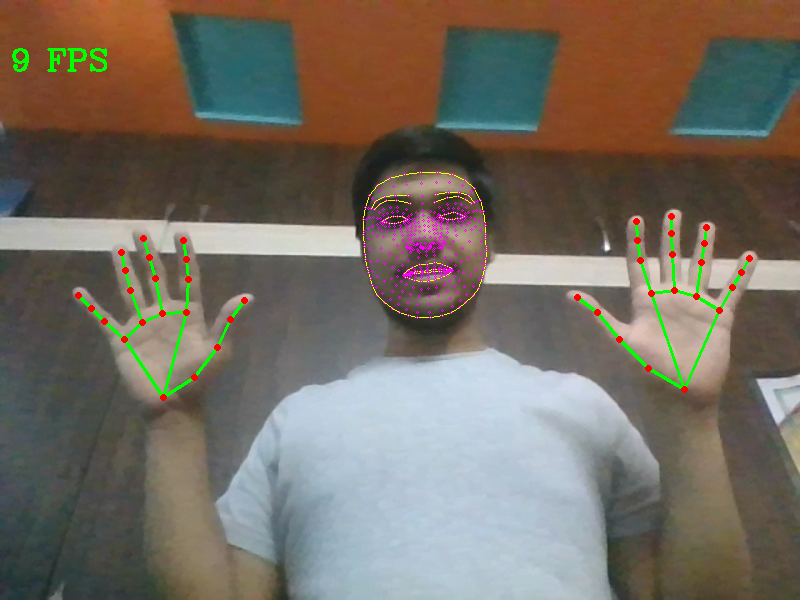
\includegraphics[width=0.85\textwidth]{figures/gloss-recognition/mediapipe-intuition.png}
  \caption{Intuicja stojąca za ekstrakcją punktów charakterystycznych za pomocą MediaPipe.}
  \label{fig:mediapipe-intuition}
\end{figure}

\begin{figure}[htbp]
  \centering
  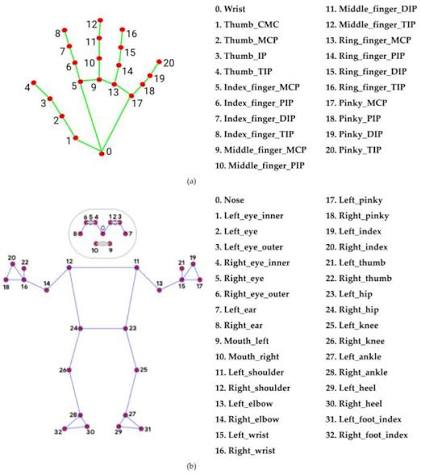
\includegraphics[width=0.7\textwidth]{figures/gloss-recognition/mediapipe-holistic-landmarks.png}
  \caption{Układ punktów charakterystycznych MediaPipe Holistic (poza, twarz i dłonie).}
  \label{fig:mediapipe-holistic-landmarks}
\end{figure}

Proces przetwarzania wstępnego przebiega w następujących etapach:

\begin{enumerate}
  \item \textbf{Sprawdzenie aktywności dłoni} -- obecność dłoni jest oceniana
        w całej sekwencji; jeśli dana dłoń jest nieobecna w większości klatek,
        jej współrzędne punktów charakterystycznych są zastępowane pozycją
        odpowiadającego jej stawu barkowego w tych klatkach. Zapewnia to modelowi
        stabilny, zakotwiczony anatomicznie punkt zastępczy zamiast eksponowania
        go na w dużej mierze brakujący tor współrzędnych, który w przeciwnym
        razie mógłby prowadzić do powstawania przypadkowych gradientów lub
        zaburzać interpolację czasową;
  \item \textbf{Interpolacja czasowa} -- współrzędne punktów charakterystycznych
        brakujące w pojedynczych klatkach (ale nie w większości sekwencji) są
        odzyskiwane za pomocą interpolacji liniowej wzdłuż osi czasu; tory
        współrzędnych brakujące całkowicie, a więc niemożliwe do interpolacji,
        są wypełniane zerami;
  \item \textbf{Usuwanie klatek statycznych} -- klatki wnoszące pomijalny ruch
        są identyfikowane i usuwane poprzez progowanie wartości przemieszczenia
        punktów charakterystycznych pomiędzy kolejnymi klatkami, dzięki czemu
        enkoder czasowy koncentruje się na dynamice istotnej dla gestu;
  \item \textbf{Wygładzanie} -- pozostała sekwencja jest wygładzana za pomocą
        filtru Savitzky'ego-Golaya, który tłumi wysokoczęstotliwościowe drgania
        punktów charakterystycznych wynikające z szumu detekcji MediaPipe, przy
        jednoczesnym zachowaniu zasadniczego przebiegu ruchu;
  \item \textbf{Normalizacja przestrzenna} -- współrzędne punktów
        charakterystycznych są normalizowane poprzez przesunięcie początku
        układu współrzędnych do punktu środkowego pomiędzy dwoma barkami oraz
        przeskalowanie względem odległości między barkami, dzięki czemu
        reprezentacja staje się niezmienna względem bezwzględnego położenia
        osoby migającej i jej fizycznej skali w kadrze;
  \item \textbf{Próbkowanie czasowe} -- każda wstępnie przetworzona sekwencja
        jest ponownie próbkowana do stałej długości 60 klatek za pomocą
        interpolacji, zapewniając jednakową długość wejścia dla wszystkich
        próbek niezależnie od pierwotnego czasu trwania nagrania.
\end{enumerate}

\subsection{Architektura modelu}
\label{sec:gloss-recognition-model}

Dla pełnego nagrania gestu każda klatka jest przetwarzana za pomocą MediaPipe
w celu wyodrębnienia punktów charakterystycznych szkieletu obejmujących pozę
ciała, dłonie i twarz. Aby uzyskać reprezentacje niezmienne względem pozy
i wyeliminować zależność od bezwzględnego położenia ciała w kadrze, współrzędne
punktów charakterystycznych są normalizowane, a każdy zestaw punktów dla
pojedynczej klatki jest spłaszczany do ciągłego wektora $\mathbb{R}^L$, gdzie
$L$ oznacza całkowitą liczbę współrzędnych punktów charakterystycznych.
Spłaszczenie usuwa jawną strukturę topologiczną grafu szkieletu -- anatomiczne
połączenia pomiędzy punktami (np. fakt, że nadgarstek jest stawem nadrzędnym
względem kości śródręcza) -- dlatego model musi w sposób niejawny wnioskować
o relacjach przestrzennych pomiędzy punktami zamiast korzystać z nich jako
ze strukturalnie zakodowanej informacji; ograniczenie to omówiono ponownie
w Sekcji~\ref{sec:gloss-recognition-discussion}.

Powstała sekwencja wektorów reprezentujących poszczególne klatki jest najpierw
rzutowana do przestrzeni o wyższym wymiarze za pomocą warstwy liniowej
rozłożonej w czasie -- pojedynczej warstwy gęstej stosowanej niezależnie
i identycznie w każdym kroku czasowym -- a następnie przekazywana do enkodera
czasowego, który może być zrealizowany jako Transformer, LSTM, GRU, BiLSTM
lub BiGRU (Rysunek~\ref{fig:model-architecture}). Enkoder działa na całym
zakresie czasowym sekwencji, generując sekwencję osadzeń uwzględniających
kontekst czasowy, po jednym dla każdej klatki wejściowej.

\begin{figure}[htbp]
  \centering
  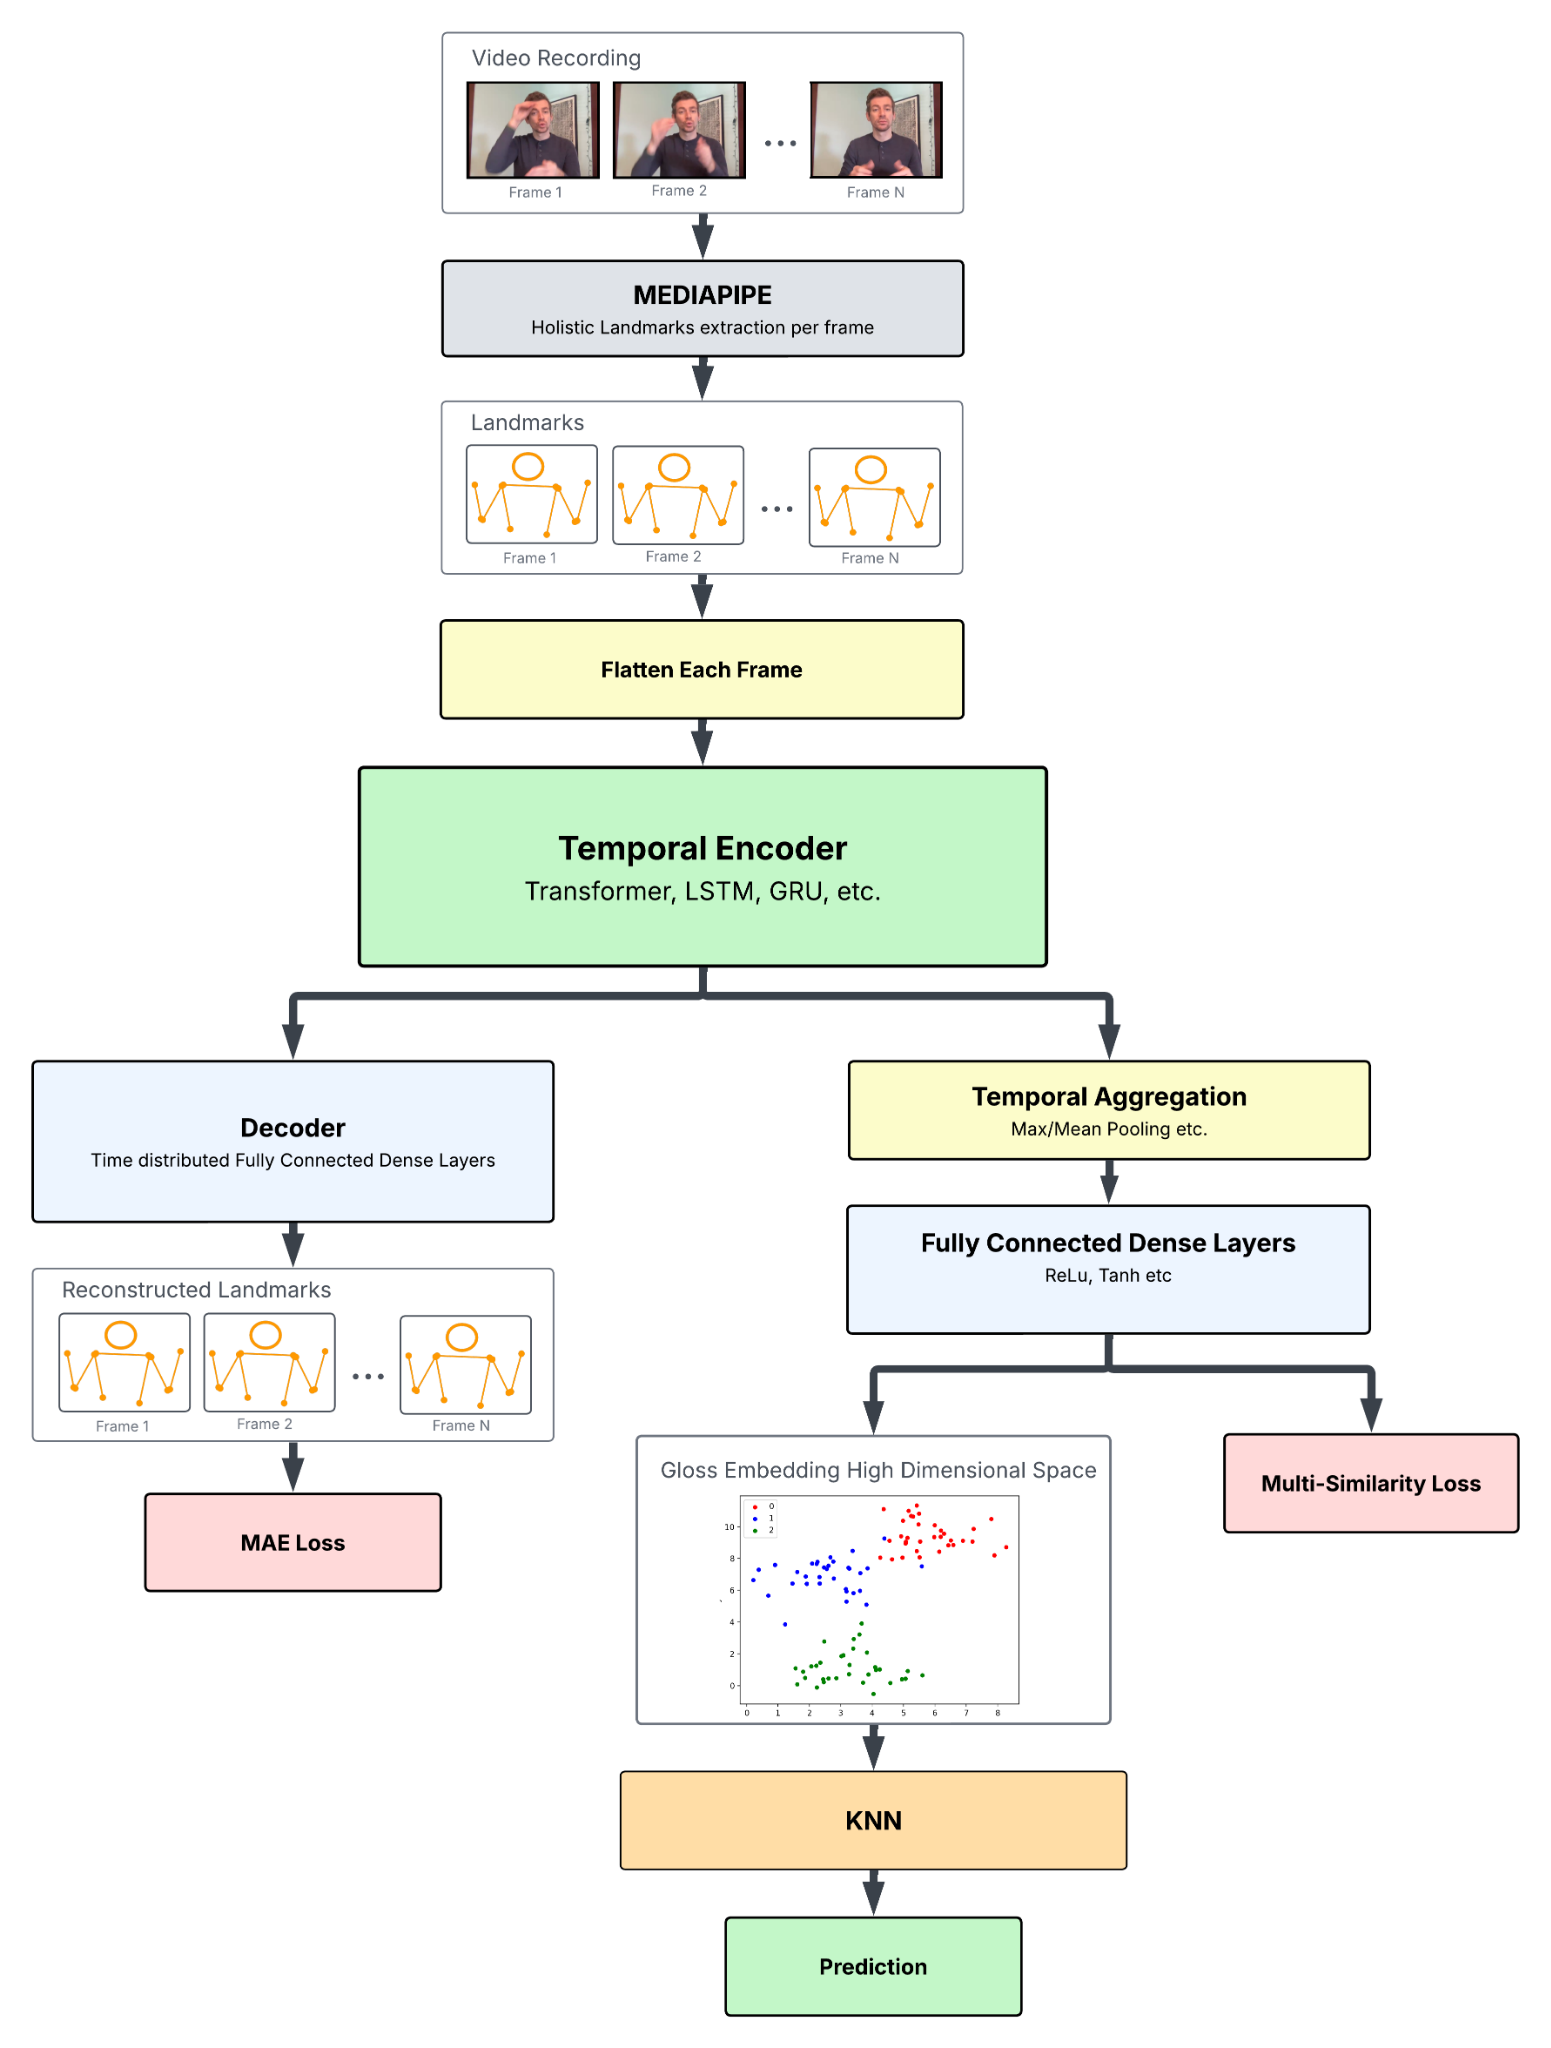
\includegraphics[width=0.85\textwidth]{figures/gloss-recognition/model-architecture.png}
  \caption{Ogólna architektura proponowanego modelu rozpoznawania
  video-to-gloss opartego na wyszukiwaniu.}
  \label{fig:model-architecture}
\end{figure}

\subsubsection{Enkodery czasowe}

Enkoder LSTM przetwarza sekwencję wejściową autoregresyjnie w kierunku zgodnym
z osią czasu (Rysunek~\ref{fig:lstm-cell}). W każdym kroku czasowym $t$ komórka
LSTM otrzymuje bieżące rzutowane osadzenie $x_t$ wraz ze stanem ukrytym
$h_{t-1}$ oraz stanem komórki $c_{t-1}$ przeniesionymi z poprzedniego kroku,
a następnie generuje zaktualizowany stan ukryty $h_t$. Stan komórki pełni
funkcję mechanizmu pamięci długoterminowej, umożliwiając sieci selektywne
zachowywanie lub odrzucanie informacji pomiędzy dowolnie odległymi krokami
czasowymi za pomocą mechanizmu bramek. BiLSTM rozszerza tę koncepcję poprzez
uruchomienie dwóch niezależnych łańcuchów LSTM dla tej samej sekwencji,
jednego w kierunku zgodnym z osią czasu i drugiego w kierunku przeciwnym,
a następnie połączenie ich wyjść w każdej pozycji $t$ w jeden stan ukryty
$h_t = [h_t^{\rightarrow}; h_t^{\leftarrow}]$, dzięki czemu model może
uwzględniać zarówno kontekst przeszły, jak i przyszły względem danej pozycji.

\begin{figure}[htbp]
  \centering
  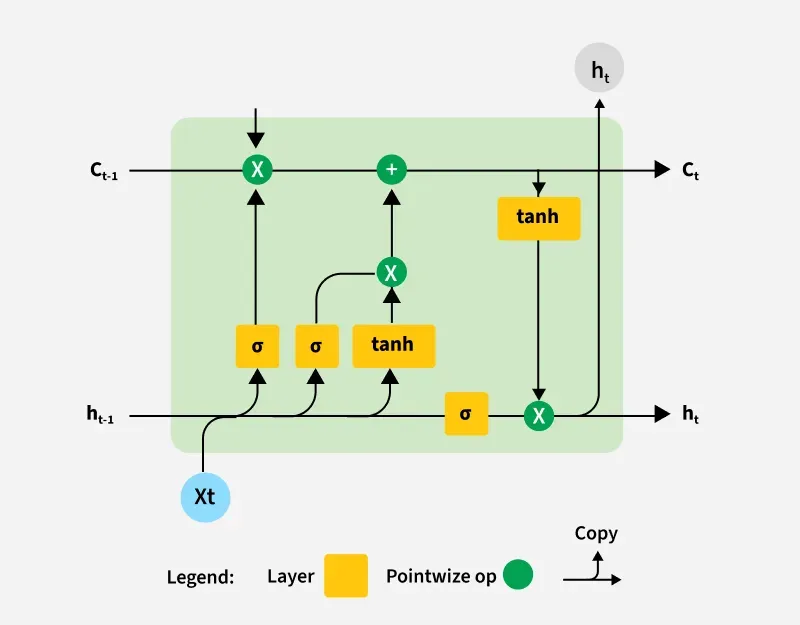
\includegraphics[width=0.6\textwidth]{figures/gloss-recognition/lstm-cell.png}
  \caption{Komórka LSTM (po lewej) oraz jej dwukierunkowe rozszerzenie BiLSTM (po prawej).}
  \label{fig:lstm-cell}
\end{figure}

Enkoder GRU również przetwarza sekwencję wejściową w kierunku zgodnym z osią
czasu, lecz upraszcza komórkę LSTM poprzez zastąpienie oddzielnych stanów
ukrytego i komórki jednym zunifikowanym stanem ukrytym $h_t$
(Rysunek~\ref{fig:gru-cell}). Zamiast bramki wejściowej, bramki zapominania
i bramki wyjściowej GRU wykorzystuje bramkę aktualizacji $z_t$, która
kontroluje, jaka część poprzedniego stanu ukrytego jest przekazywana dalej,
oraz bramkę resetowania $r_t$, określającą, w jakim stopniu wcześniejszy
kontekst wpływa na kandydacki stan ukryty. Zredukowana liczba parametrów
sprawia, że GRU jest mniej wymagający obliczeniowo niż LSTM, zachowując
jednocześnie zdolność modelowania długoterminowych zależności czasowych.
BiGRU stosuje tę samą zasadę rozszerzenia co BiLSTM, uruchamiając dwa
niezależne łańcuchy GRU w przeciwnych kierunkach i łącząc ich wyjścia
w każdym kroku czasowym.

\begin{figure}[htbp]
  \centering
  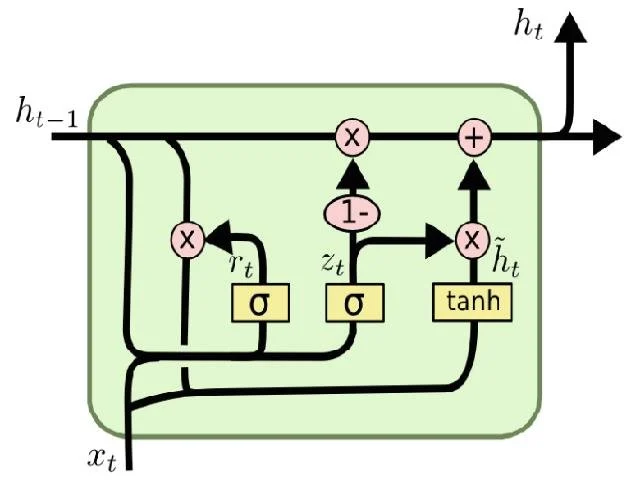
\includegraphics[width=0.6\textwidth]{figures/gloss-recognition/gru-cell.png}
  \caption{Komórka GRU (po lewej) oraz jej dwukierunkowe rozszerzenie BiGRU (po prawej).}
  \label{fig:gru-cell}
\end{figure}

Enkoder Transformer zasadniczo różni się od podejścia rekurencyjnego:
przetwarza wszystkie kroki czasowe równolegle, a nie jeden po drugim
(Rysunek~\ref{fig:transformer-encoder}). Ponieważ architektura jest z natury
niezmiennicza względem permutacji, przed przetwarzaniem do rzutowanych
osadzeń wejściowych dodawane są jawne kodowania pozycji. Podstawową jednostką
obliczeniową jest skalowana samouwaga oparta na iloczynie skalarnym
(scaled dot-product self-attention): w każdej warstwie każda pozycja $t$
wyznacza zapytanie $q_t$, zbiór kluczy $\{k_1, \ldots, k_T\}$ oraz zbiór
wartości $\{v_1, \ldots, v_T\}$ poprzez nauczalne projekcje liniowe wejścia,
a wyjście dla pozycji $t$ jest ważoną sumą wszystkich wektorów wartości,
gdzie waga przypisana pozycji $s$ jest proporcjonalna do
$\exp(q_t^\top k_s / \sqrt{d_k})$, przy czym $d_k$ oznacza wymiar klucza.
Każda pozycja może zatem bezpośrednio uwzględniać każdą inną pozycję już
w pojedynczej warstwie, zapewniając Transformerowi globalne pole percepcji
od pierwszej warstwy -- właściwość, której LSTM ani GRU nie posiadają bez
zwiększania głębokości. Samouwaga jest obliczana równolegle dla $H$
niezależnych głów, których wyjścia są następnie łączone i rzutowane liniowo;
po każdej podwarstwie samouwagi następuje pozycjonowana sieć
feed-forward, a obie podwarstwy są otoczone połączeniami rezydualnymi
i normalizacją warstwy.

\begin{figure}[htbp]
  \centering
  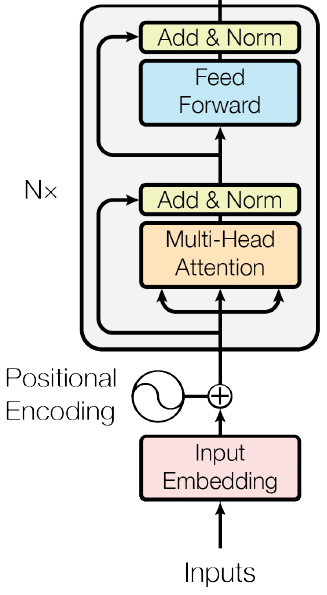
\includegraphics[width=0.6\textwidth]{figures/gloss-recognition/transformer-encoder.png}
  \caption{Enkoder Transformer.}
  \label{fig:transformer-encoder}
\end{figure}

\subsubsection{Dekoder rekonstrukcyjny, agregacja i wyszukiwanie}

Wyjście enkodera jest kierowane do dwóch równoległych gałęzi. Pierwsza z nich,
dekoder rekonstrukcyjny -- stos warstw gęstych rozłożonych w czasie -- próbuje
odtworzyć oryginalne wektory punktów charakterystycznych dla poszczególnych
klatek na podstawie ich zakodowanych reprezentacji. Ten pomocniczy cel pełni
funkcję mechanizmu regularyzacyjnego: wymagając od enkodera zachowania
wystarczającej ilości informacji do rekonstrukcji wejścia, ogranicza ryzyko
załamania reprezentacji i sprzyja uczeniu gęstych osadzeń wiernych geometrii.
Co istotne, tworzy to również podstawę dla planowanego rozszerzenia potoku
wyszukiwania: ponieważ nauczone osadzenia pozostają zakotwiczone w strukturze
pierwotnej przestrzeni punktów charakterystycznych, dobrze nadają się do
wyrównywania sekwencji z wykorzystaniem Dynamic Time Warping (DTW),
omówionego szerzej w Sekcji~\ref{sec:gloss-recognition-discussion}.

Druga gałąź stosuje agregację czasową -- Global Mean Pooling wzdłuż wymiaru
czasowego wyjścia enkodera, obliczając średnią elementową dla wszystkich
$T$ kroków czasowych w celu uzyskania pojedynczego wektora o stałej długości
$z \in \mathbb{R}^d$ -- a następnie stos w pełni połączonych warstw gęstych,
które nieliniowo rzutują $z$ do wysokowymiarowej przestrzeni osadzeń. Ta
końcowa projekcja nie podejmuje bezpośrednio decyzji klasyfikacyjnej;
jej wyjściem jest ciągły wektor osadzenia stanowiący przestrzeń wejściową
dla klasyfikatora $k$ najbliższych sąsiadów (KNN). Warstwy gęste są więc
trenowane nie po to, aby bezpośrednio rozróżniać klasy glos, lecz aby
kształtować geometrię przestrzeni osadzeń tak, by osadzenia tej samej glosy
tworzyły zwarte skupiska, podczas gdy osadzenia różnych glos były od siebie
oddalane. Klasyfikacja jest w całości delegowana do KNN, który wyszukuje
$k$ najbardziej podobnych osadzeń w oznaczonym zbiorze referencyjnym
i określa przewidywaną glosę na podstawie głosowania większościowego
wśród ich etykiet.

\subsubsection{Złożona funkcja straty}

Aby narzucić pożądaną strukturę geometryczną przestrzeni osadzeń, przyjmujemy
funkcję straty Multi-Similarity (MS) \cite{wang2019msloss} jako cel uczenia
metrycznego. W przeciwieństwie do prostszych funkcji kontrastowych lub
triplet loss, które rozpatrują pojedyncze pary lub trójki niezależnie,
MS loss operuje na pełnej strukturze podobieństwa par w obrębie partii
treningowej. Dla każdego osadzenia bazowego $i$ definiuje zbiór par pozytywnych
$P_i$ (osadzenia mające tę samą etykietę glosy) oraz zbiór par negatywnych
$N_i$ (osadzenia należące do różnych glos), a następnie stosuje asymetryczne
ważenie obu zbiorów na podstawie podobieństw cosinusowych $S_{ik}$:

\begin{equation}
  \mathcal{L}_{MS} = \frac{1}{m}\sum_{i=1}^{m}\left\{
    \frac{1}{\alpha}\log\!\left[1+\sum_{k\in P_i}e^{-\alpha(S_{ik}-\lambda)}\right]
  + \frac{1}{\beta}\log\!\left[1+\sum_{k\in N_i}e^{\beta(S_{ik}-\lambda)}\right]
  \right\}
  \label{eq:ms-loss}
\end{equation}

gdzie $\alpha$ i $\beta$ są hiperparametrami skalującymi kontrolującymi
stromość odpowiednio wagowania pozytywnego i negatywnego, natomiast
$\lambda$ jest progiem marginesu. Łączny efekt polega na przyciąganiu do
siebie osadzeń tej samej glosy oraz odsuwaniu od siebie osadzeń różnych glos,
przy czym sygnał gradientowy koncentruje się na parach najbardziej użytecznych
z punktu widzenia rozróżniania w danej partii.

Funkcja straty MS jest addytywnie łączona z funkcją straty rekonstrukcji
Mean Squared Error (MSE), generowaną przez gałąź dekodera, która penalizuje
odchylenie pomiędzy oryginalnymi wektorami punktów charakterystycznych
$x_t$ a ich rekonstrukcjami $\hat{x}_t$:

\begin{equation}
  \mathcal{L}_{rec} = \frac{1}{T}\sum_{t=1}^{T} \lVert x_t - \hat{x}_t \rVert_2^2
  \label{eq:mse-loss}
\end{equation}

Oba cele są łączone w złożoną funkcję straty za pomocą skalarnego
hiperparametru $\gamma$, który określa względny udział składnika
rekonstrukcyjnego:

\begin{equation}
  \mathcal{L} = \mathcal{L}_{MS} + \gamma\, \mathcal{L}_{rec}
  \label{eq:composite-loss}
\end{equation}

\subsection{Eksperymenty i wyniki}
\label{sec:gloss-recognition-experiments}

\subsubsection{Procedura treningowa}

Model jest trenowany jako enkoder wykorzystujący uczenie metryczne, którego
celem jest utworzenie geometrycznie uporządkowanej przestrzeni osadzeń dla
reprezentacji gestów. Wszystkie osadzenia są normalizowane za pomocą normy L2
przed obliczeniem funkcji straty oraz podczas ewaluacji, co ogranicza przestrzeń
osadzeń do jednostkowej hipersfery i zapewnia równoważność podobieństwa
cosinusowego oraz odległości euklidesowej.

Trening wykorzystuje optymalizator Adam z początkowym współczynnikiem uczenia
$5\times10^{-4}$ oraz harmonogram Cosine Annealing with Warm Restarts
($T_0=30$, $T_{mult}=2$, $\eta_{min}=1\times10^{-6}$;
Rysunek~\ref{fig:lr-schedule}), w którym współczynnik uczenia maleje zgodnie
z krzywą cosinusoidalną od aktualnej wartości maksymalnej do $\eta_{min}$,
po czym jest okresowo ponownie zwiększany; odstęp pomiędzy kolejnymi
restartami jest podwajany po każdym cyklu. Partie treningowe są konstruowane
za pomocą próbnika $P \times K$, gdzie $P=16$ oznacza klas, a $K=4$ próbki
na klasę, co daje partie liczące do 64 próbek -- jest to strategia
zrównoważonego próbkowania klasowego, będąca warunkiem skutecznego uczenia
metrycznego, ponieważ zapewnia wystarczającą liczbę par pozytywnych
i negatywnych w każdej partii, aby funkcja MS mogła generować informatywne
gradienty. Waga złożonej funkcji straty została ustawiona na $\gamma=0.25$,
co pozwala składnikowi rekonstrukcyjnemu pełnić funkcję regularyzującą
enkoder bez zdominowania celu uczenia metrycznego.

\begin{figure}[htbp]
  \centering
  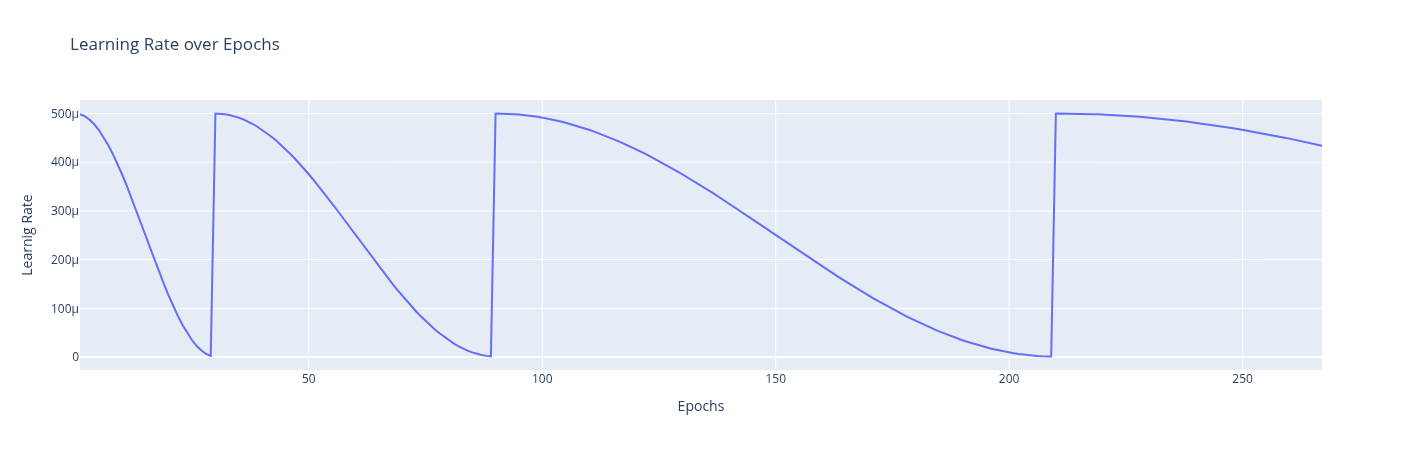
\includegraphics[width=0.65\textwidth]{figures/gloss-recognition/lr-schedule.png}
  \caption{Harmonogram współczynnika uczenia w trakcie treningu.}
  \label{fig:lr-schedule}
\end{figure}

Od epoki 30 utrzymywana jest średnia krocząca wykładnicza (EMA) wag modelu
ze współczynnikiem zaniku 0.99; od tego momentu model EMA jest używany
wyłącznie do walidacji i zapisywania checkpointów zamiast surowego stanu
parametrów, co zazwyczaj zapewnia bardziej stabilną i lepiej generalizującą
ewaluację. Wydajność modelu oceniana jest na zbiorze walidacyjnym za pomocą
dokładności 1-najbliższego sąsiada (1-NN) w nauczonej przestrzeni osadzeń --
każdej próbce walidacyjnej przypisywana jest etykieta jej pojedynczego
najbliższego sąsiada w przestrzeni osadzeń utworzonej na podstawie zbioru
treningowego. Zachowywany jest checkpoint osiągający najwyższą dokładność
1-NN, przy czym strata walidacyjna służy jako kryterium rozstrzygające
w przypadku remisu; trening podlega również wczesnemu zatrzymaniu
z cierpliwością wynoszącą 50 epok.

\subsubsection{Metryki ogólne}

Pięć wariantów enkoderów czasowych -- Transformer, LSTM, BiLSTM, GRU i BiGRU --
jest ocenianych przy identycznej konfiguracji eksperymentalnej (ten sam potok
przetwarzania wstępnego, próbnik partii, funkcja straty i harmonogram treningu),
co zapewnia, że obserwowane różnice wydajności wynikają z wyboru enkodera
czasowego, a nie z czynników zakłócających. Raportowane metryki obejmują:
\emph{accuracy} (dokładność klasyfikacji 1-NN na zbiorze walidacyjnym,
będącą główną metryką rankingową), \emph{loss} (złożony cel treningowy
w najlepszym punkcie kontrolnym walidacji), \emph{positive pair distance}
(średnia odległość osadzeń pomiędzy parami tej samej glosy; niższa wartość
jest lepsza), \emph{negative pair distance} (średnia odległość osadzeń
pomiędzy parami różnych glos; wyższa wartość jest lepsza) oraz
\emph{distance margin} (różnica pomiędzy średnią odległością par negatywnych
i pozytywnych, podsumowująca strukturę dyskryminacyjną w jednej wartości).

\begin{figure}[htbp]
  \centering
  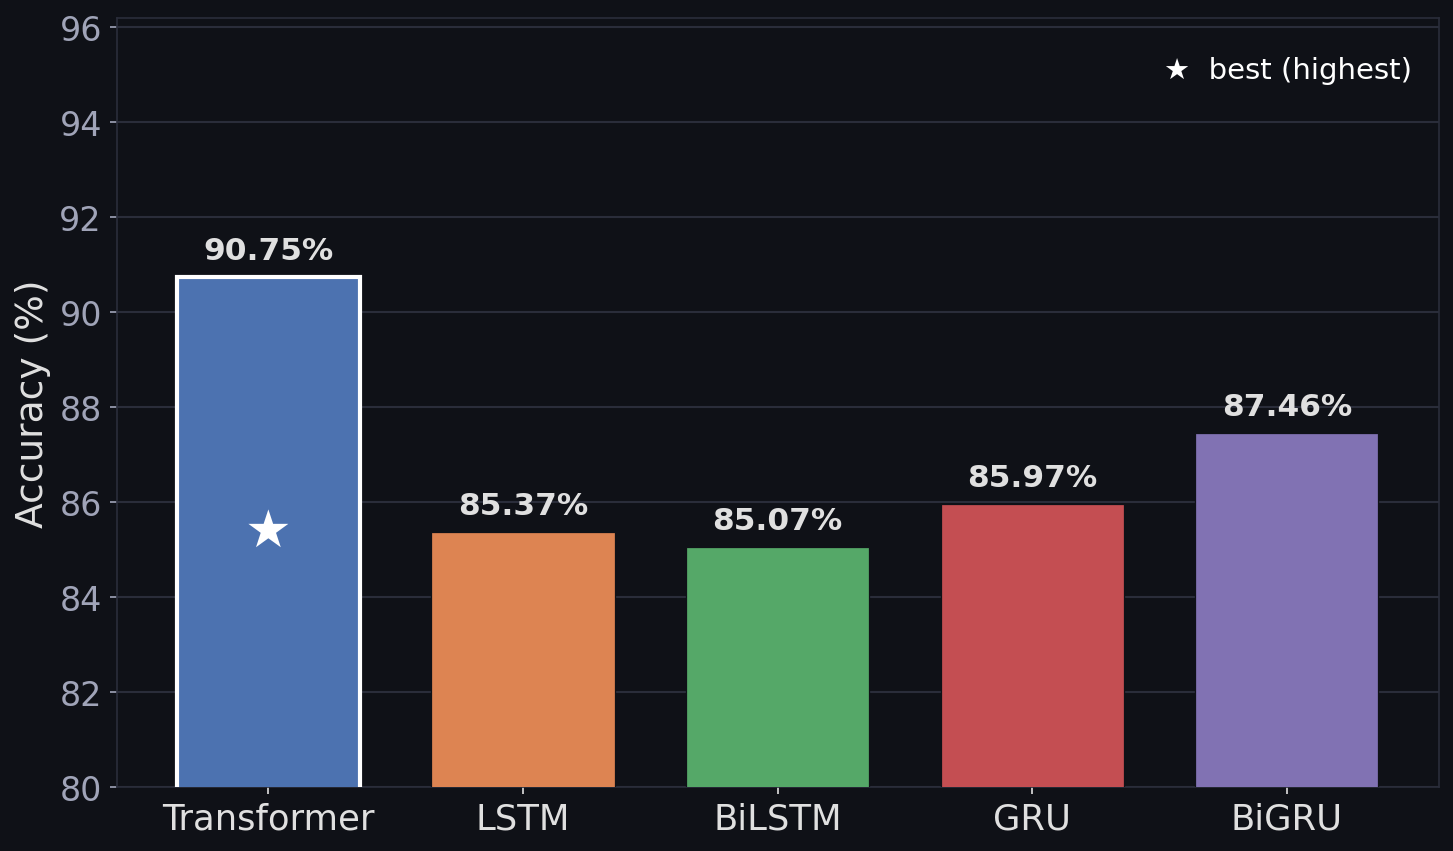
\includegraphics[width=0.48\textwidth]{figures/gloss-recognition/accuracy-validation.png}\hfill
  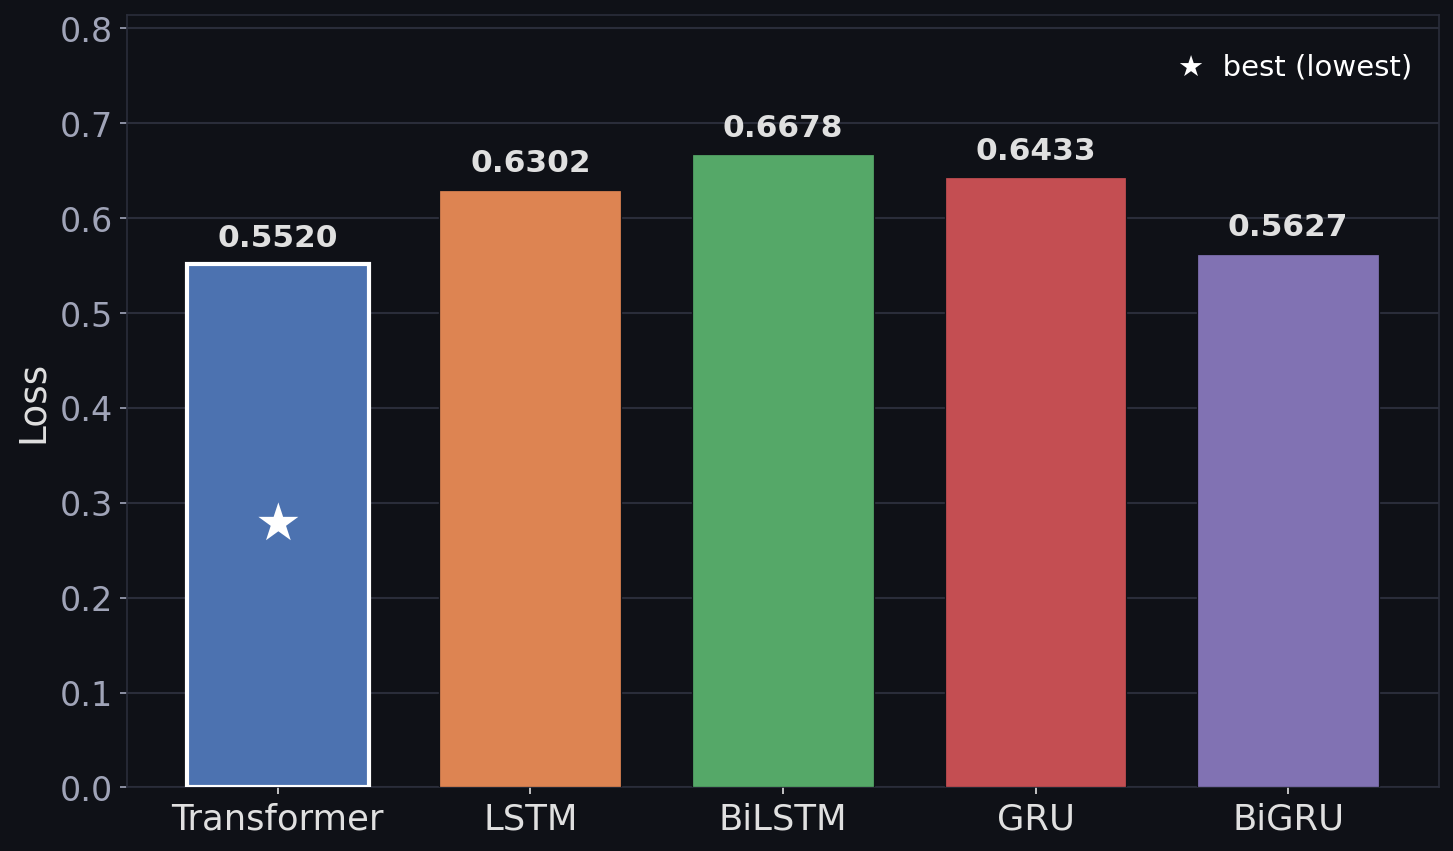
\includegraphics[width=0.48\textwidth]{figures/gloss-recognition/loss-validation.png}
  \caption{Dokładność walidacyjna (po lewej) oraz strata walidacyjna (po prawej)
  dla pięciu analizowanych enkoderów czasowych.}
  \label{fig:accuracy-loss}
\end{figure}

\begin{figure}[htbp]
  \centering
  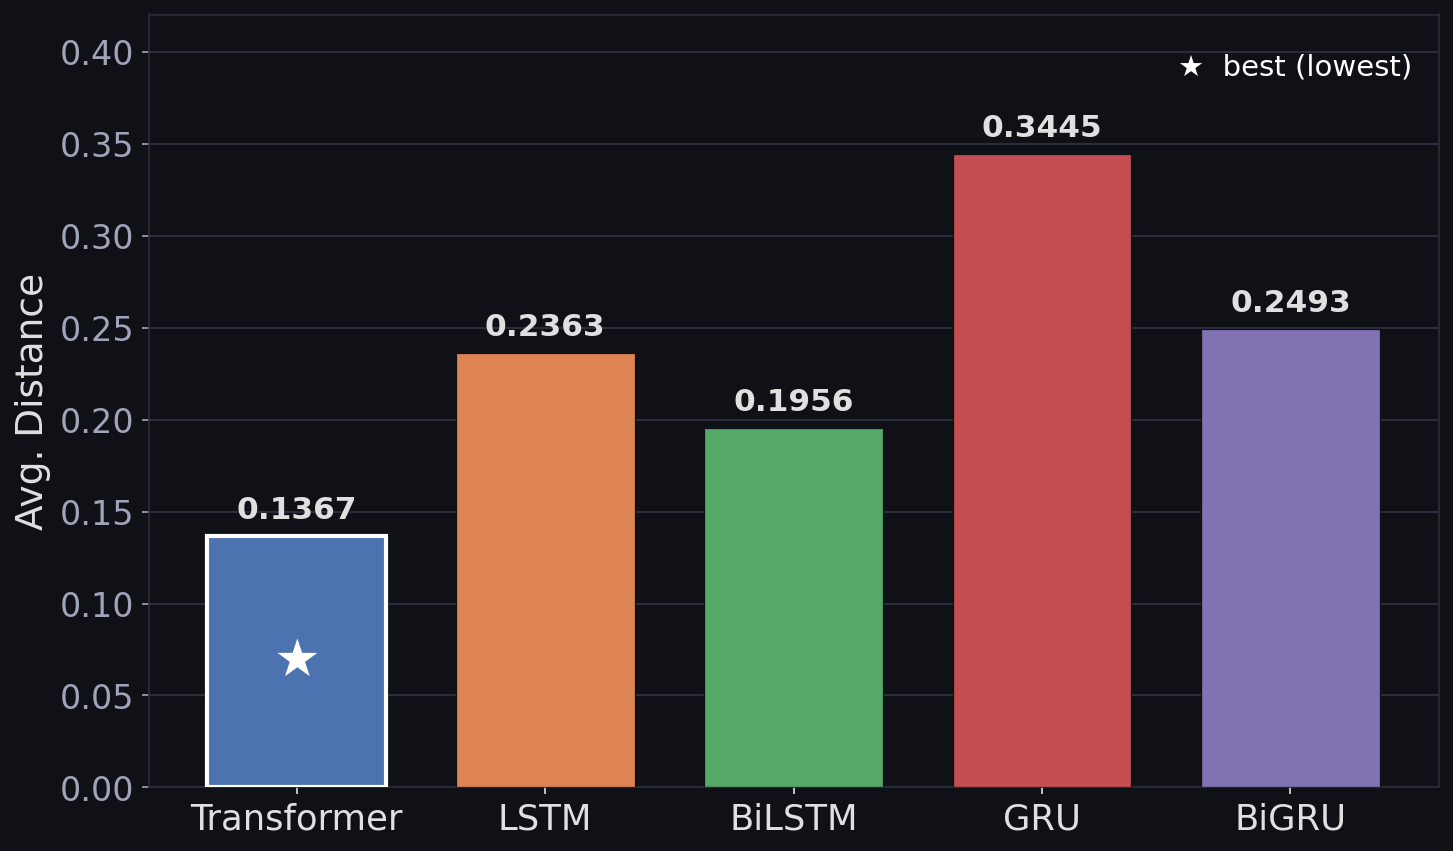
\includegraphics[width=0.32\textwidth]{figures/gloss-recognition/train-positive-distance.png}\hfill
  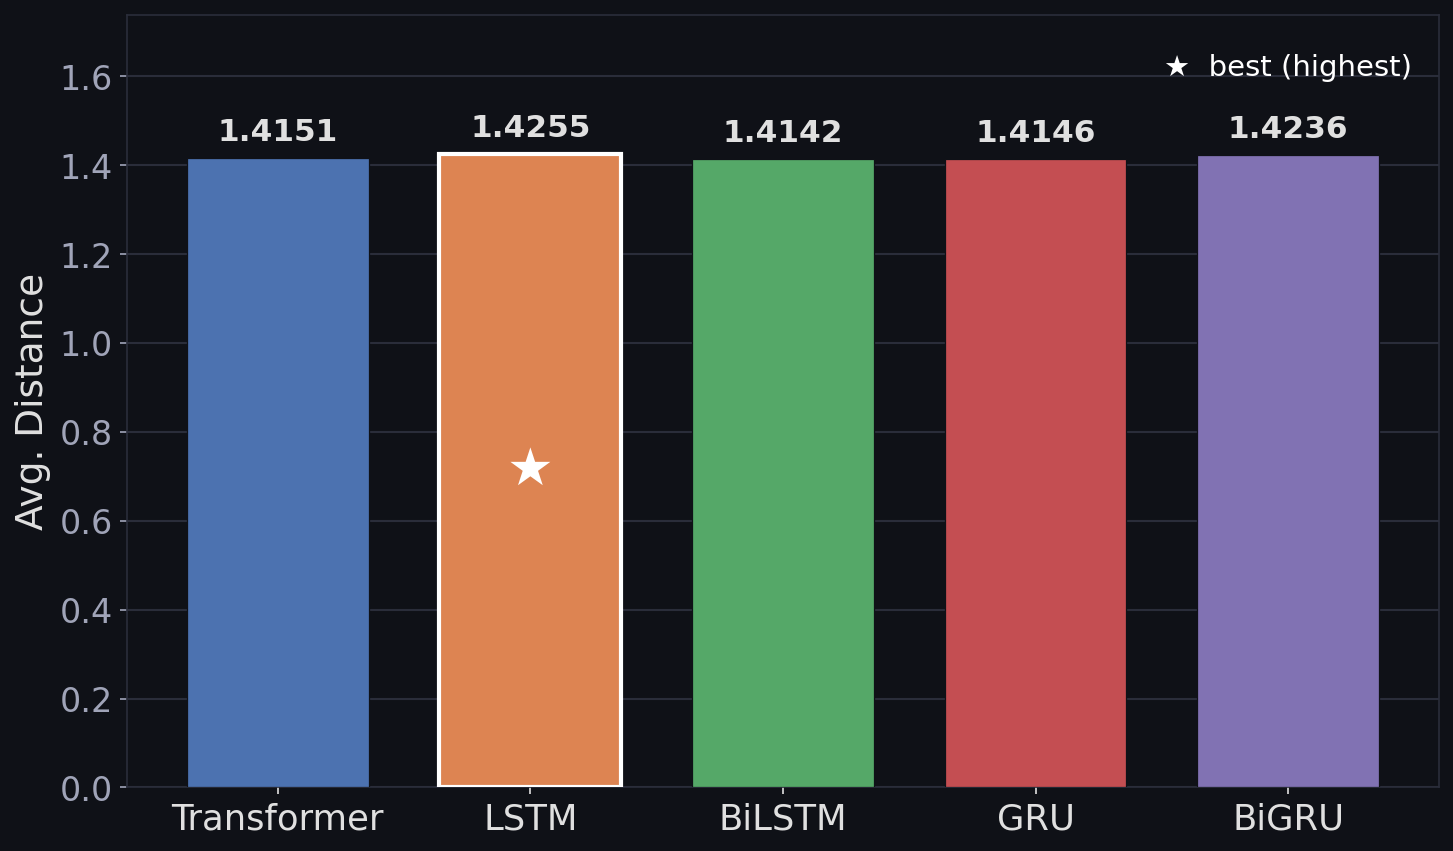
\includegraphics[width=0.32\textwidth]{figures/gloss-recognition/train-negative-distance.png}\hfill
  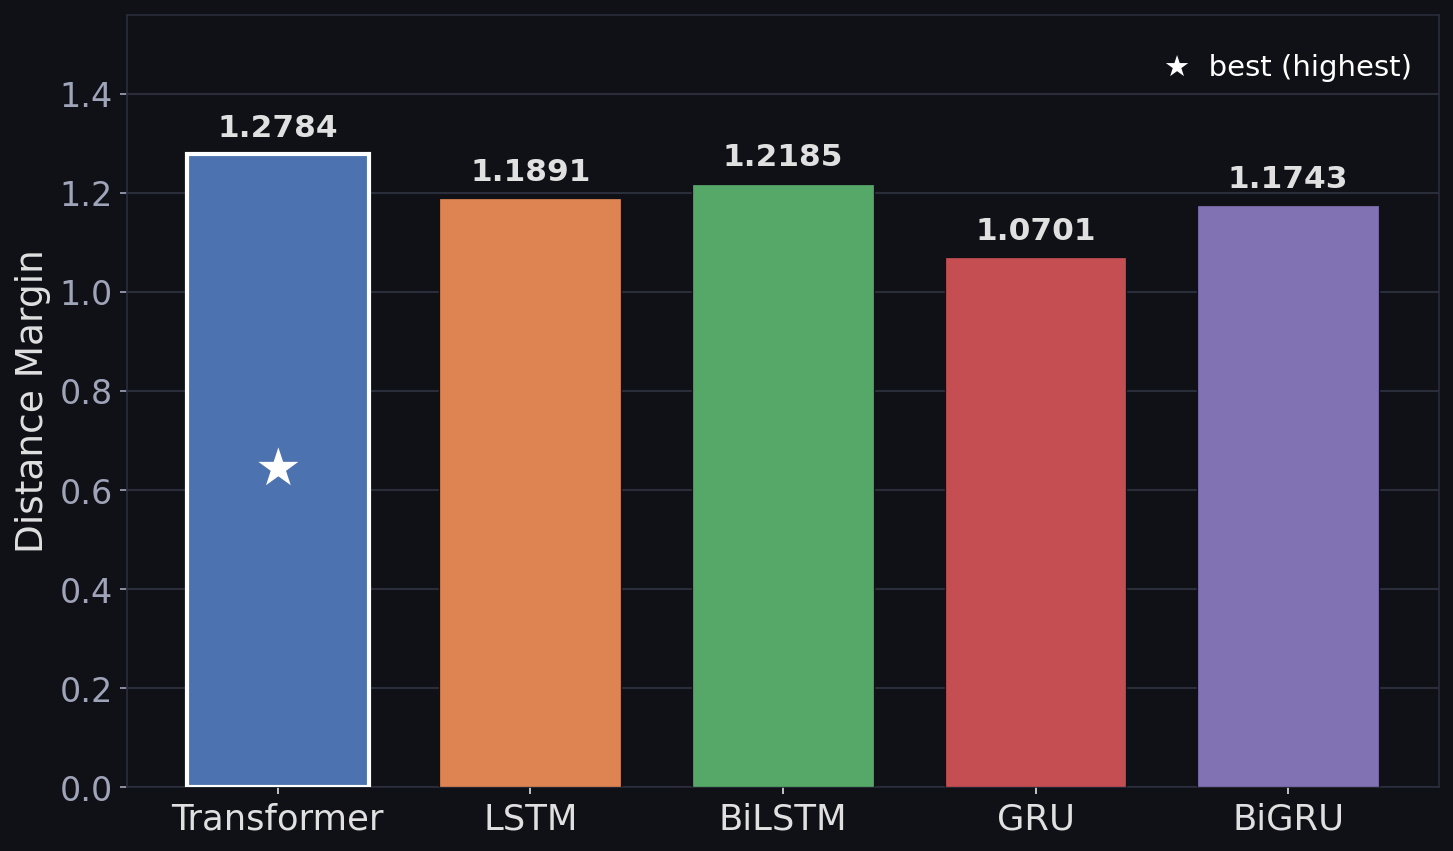
\includegraphics[width=0.32\textwidth]{figures/gloss-recognition/train-distance-margin.png}
  \caption{Odległość par pozytywnych, odległość par negatywnych oraz margines
  odległości (trening vs.\ walidacja) dla pięciu analizowanych enkoderów czasowych.}
  \label{fig:distance-metrics}
\end{figure}

Jak przedstawiono na Rysunkach~\ref{fig:accuracy-loss} i
\ref{fig:distance-metrics}, enkoder Transformer osiąga najlepsze wyniki
w większości raportowanych metryk, uzyskując najwyższą dokładność 1-NN
(\textbf{90.75\%}), najniższą złożoną funkcję straty, największy margines
odległości oraz najmniejszą odległość par pozytywnych. Jedynym wyjątkiem
jest średnia odległość par negatywnych, dla której Transformer jest
nieznacznie wyprzedzany przez enkodery BiGRU i LSTM; różnica ta jest jednak
pomijalnie mała i nie wpływa znacząco na ogólny ranking. Łącznie wyniki te
wskazują, że Transformer jest najbardziej skutecznym enkoderem czasowym
w ramach proponowanej architektury. Cała dalsza analiza jest zatem
prowadzona wyłącznie z wykorzystaniem enkodera Transformer.

\todo{PLACEHOLDER: Wstawić dokładne wartości dokładności 1-NN, straty,
odległości par pozytywnych/negatywnych oraz marginesu odległości dla enkoderów
LSTM, BiLSTM, GRU i BiGRU (w raporcie źródłowym dostępna była jedynie wartość
90.75\% dokładności Transformera), aby uzupełnić tabelę porównawczą.}

\subsection{Analiza i dyskusja}
\label{sec:gloss-recognition-discussion}

Następnie przedstawiamy pogłębioną analizę kompletnego proponowanego systemu,
wykorzystując Transformer jako enkoder czasowy. Macierz pomyłek
(Rysunek~\ref{fig:confusion-matrix}) nie wykazuje systematycznego obciążenia
pomiędzy klasami -- brak dowodów na to, że model konsekwentnie myli jedną
konkretną glosę z inną. Zamiast tego obserwowane błędne klasyfikacje są
rozłożone nieregularnie pomiędzy parami glos, co sugeruje, że błędy wynikają
ze zmienności wewnątrzklasowej danych wejściowych, a nie ze strukturalnej
niejednoznaczności przestrzeni osadzeń: ta sama glosa jest często wykonywana
w różny sposób przez różne osoby migające, z różnicami w kształcie dłoni,
trajektorii ruchu i tempie migania, co odzwierciedla naturalną koartykulację
i zmienność stylistyczną charakterystyczną dla produkcji języka migowego.
Zmienność wynikająca z osoby migającej jest dobrze znanym wyzwaniem
w rozpoznawaniu izolowanych znaków i uzasadnia zastosowanie celu uczenia
metrycznego, który lepiej nadaje się do obsługi rozrzutu wewnątrzklasowego
niż klasyfikator softmax o stałych granicach klas.

\begin{figure}[htbp]
  \centering
  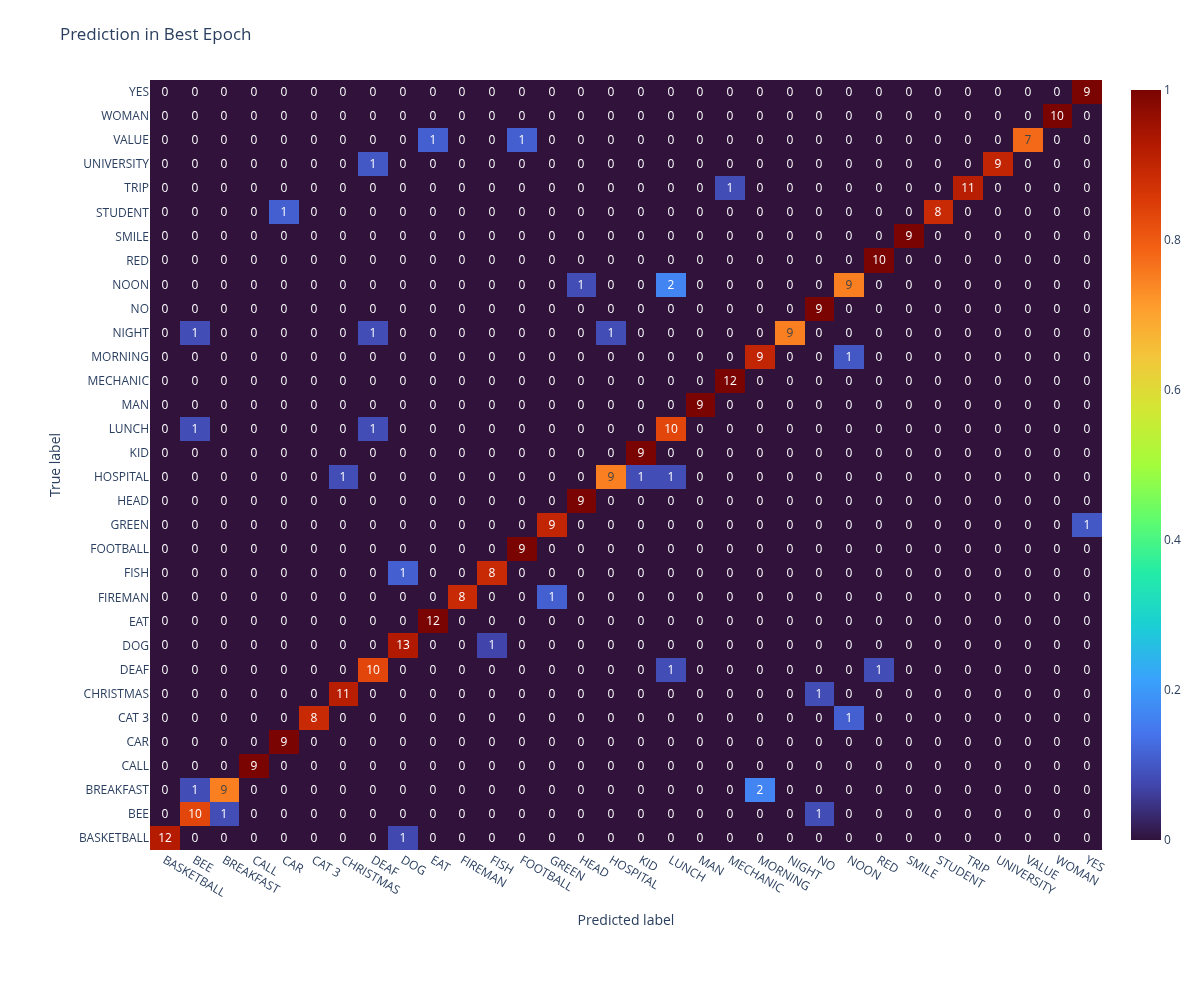
\includegraphics[width=0.6\textwidth]{figures/gloss-recognition/confusion-matrix.png}
  \caption{Macierz pomyłek dla zbioru walidacyjnego obejmującego 32 glosy
  (enkoder Transformer).}
  \label{fig:confusion-matrix}
\end{figure}

Czułość dla poszczególnych klas we wszystkich 32 glosach
(Rysunek~\ref{fig:recall-per-class}) pokazuje, że wszystkie klasy osiągają
czułość przekraczającą 0.75, co świadczy o stabilnej jakości wyszukiwania
w całym zakresie ocenianego słownictwa, obejmującym zarówno znaki wyraźnie
odróżniające się wizualnie, jak i potencjalnie niejednoznaczne. Znaczna liczba
glos osiąga idealną czułość równą 1.0. Brak jakiejkolwiek klasy poniżej progu
0.75 jest istotny, ponieważ sugeruje, że model nie wykazuje charakterystycznego
dla niezrównoważonych lub silnie zmiennych zbiorów załamania jakości dla
poszczególnych klas, w którym klasy mniejszościowe lub wizualnie podobne
są często poświęcane na rzecz ogólnej dokładności.

\begin{figure}[htbp]
  \centering
  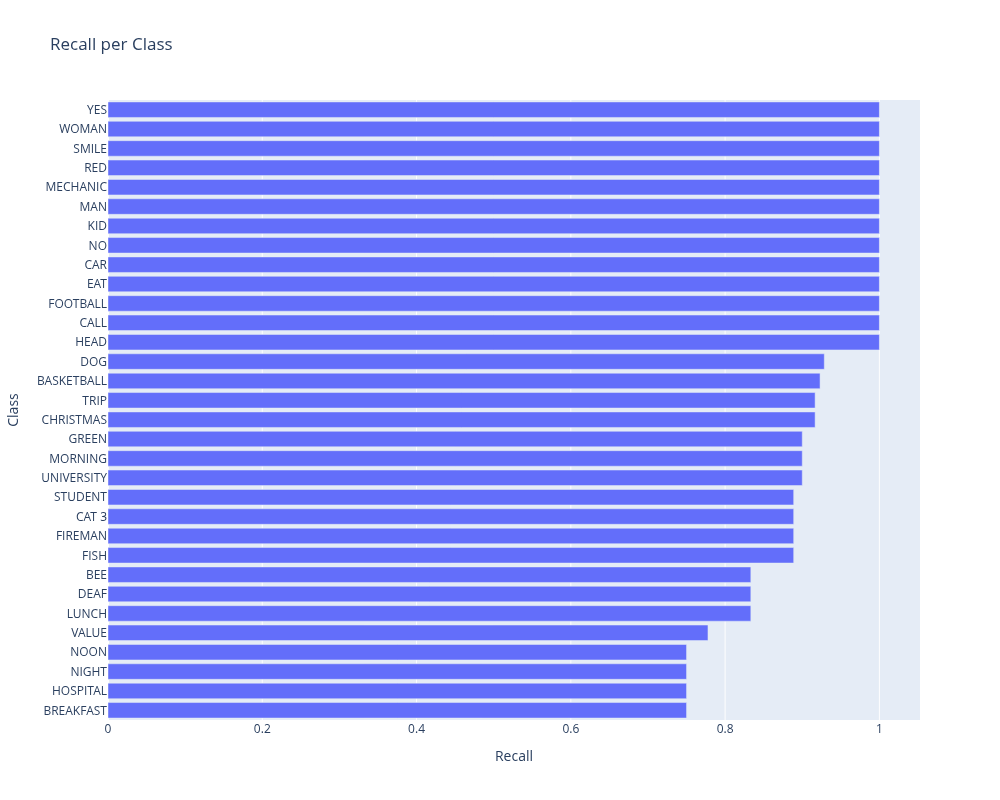
\includegraphics[width=0.6\textwidth]{figures/gloss-recognition/recall-per-class.png}
  \caption{Czułość dla poszczególnych klas dla 32 ocenianych glos
  (enkoder Transformer).}
  \label{fig:recall-per-class}
\end{figure}

Jakość geometryczną nauczonej przestrzeni osadzeń oceniamy poprzez wizualizację
osadzeń Transformera dla zbiorów treningowego i walidacyjnego za pomocą t-SNE
(t-Distributed Stochastic Neighbour Embedding), które zachowuje lokalną
strukturę sąsiedztwa i dobrze nadaje się do ujawniania geometrii skupisk.
Przestrzeń osadzeń zbioru treningowego (Rysunek~\ref{fig:tsne-training})
wykazuje dobrze zdefiniowane, niepokrywające się skupiska -- po jednym dla
każdej glosy -- o wysokiej zwartości wewnątrzklasowej, potwierdzając, że
złożona funkcja straty skutecznie ukształtowała przestrzeń osadzeń tak, aby
odzwierciedlała tożsamość glos. Przestrzeń osadzeń zbioru walidacyjnego
(Rysunek~\ref{fig:tsne-validation}) zachowuje ogólną strukturę skupisk
obserwowaną podczas treningu -- wszystkie 32 glosy pozostają rozdzielne --
jednak skupiska są zauważalnie bardziej rozproszone, a na ich granicach
występuje pewien stopień nakładania się klas. Ta rozbieżność pomiędzy geometrią
zbioru treningowego i walidacyjnego jest zgodna z omówioną wcześniej
zmiennością wewnątrzklasową: model nauczył się zwartej reprezentacji instancji
każdej glosy obecnych w treningu, lecz nieznane osoby migające wprowadzają
zmienność powodującą przesuwanie się niektórych osadzeń walidacyjnych
w kierunku granic sąsiednich skupisk. Co istotne, zachowanie globalnie
spójnej struktury skupisk w przestrzeni walidacyjnej potwierdza, że model
nauczył się generalizowalnych reprezentacji glos, zamiast przeuczyć się
na konkretne osoby migające obecne w zbiorze treningowym.

\begin{figure}[htbp]
  \centering
  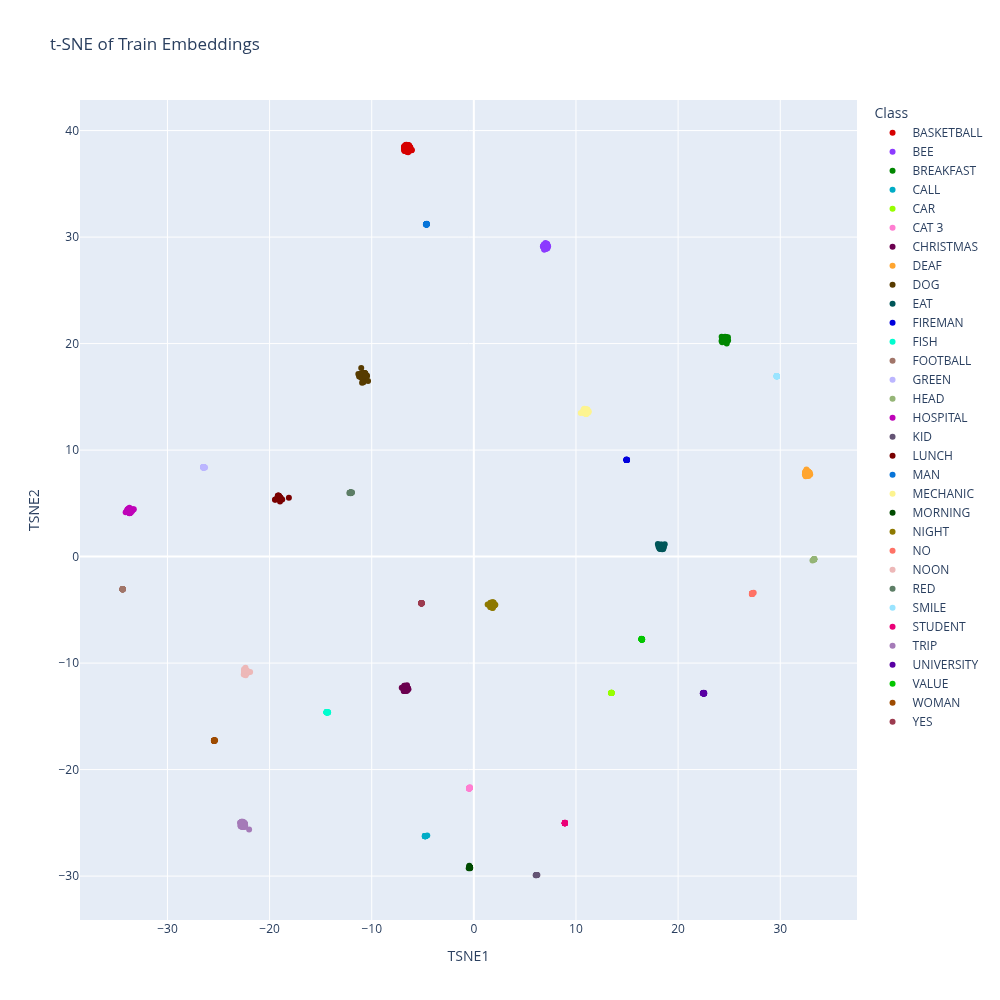
\includegraphics[width=0.48\textwidth]{figures/gloss-recognition/tsne-training.png}\hfill
  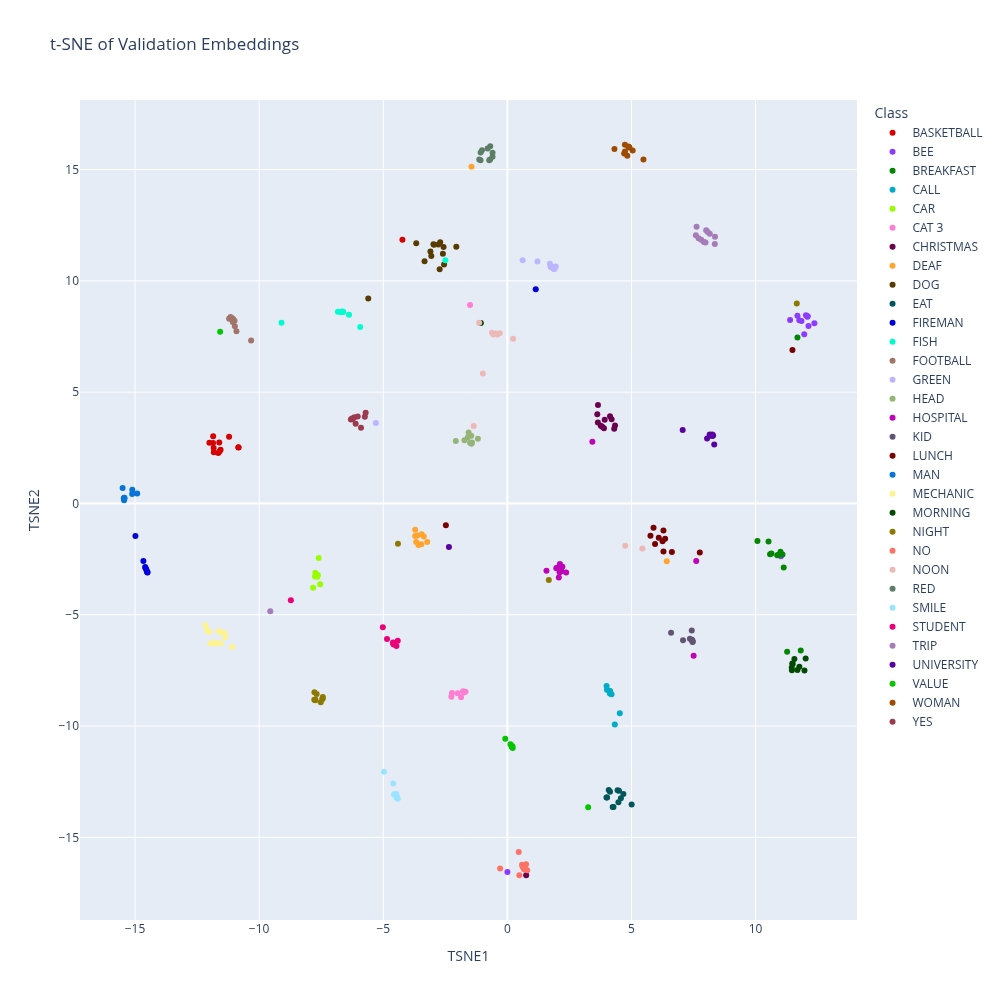
\includegraphics[width=0.48\textwidth]{figures/gloss-recognition/tsne-validation.png}
  \caption{Wizualizacja t-SNE nauczonej przestrzeni osadzeń dla zbioru
  treningowego (po lewej) i walidacyjnego (po prawej).}
  \label{fig:tsne-training}
  \label{fig:tsne-validation}
\end{figure}

Na koniec analizujemy ewolucję średnich odległości par pozytywnych
i negatywnych pod wpływem funkcji MS w trakcie treningu
(Rysunek~\ref{fig:pos-neg-distances}). Odległość par negatywnych szybko rośnie
we wczesnych etapach treningu, a następnie stabilizuje się na niezmiennie
wysokim poziomie, przy czym krzywe treningowa i walidacyjna pozostają przez
cały czas blisko siebie, wskazując, że model niezawodnie uczy się rozdzielać
osadzenia różnych glos w sposób dobrze generalizujący na niewidziane próbki.
Odległość par pozytywnych systematycznie maleje podczas treningu, odzwierciedlając
postępujące zagęszczanie skupisk wewnątrzklasowych; jednocześnie utrzymuje się
stała różnica pomiędzy krzywymi treningową i walidacyjną, przy czym walidacyjne
odległości par pozytywnych pozostają konsekwentnie wyższe. Rozbieżność ta jest
bezpośrednim przejawem omówionej wcześniej zmienności wewnątrzklasowej:
podczas gdy model skutecznie zagęszcza osadzenia instancji każdej glosy
w zbiorze treningowym, nieznane osoby migające w zbiorze walidacyjnym
wprowadzają różnice w wykonaniu, na które model nie był wcześniej wystawiony,
powodując większe rozproszenie ich osadzeń wewnątrz skupiska. Różnica ta
kwantyfikuje zatem w geometrii przestrzeni osadzeń podstawowe wyzwanie,
jakim jest zmienność zależna od osoby migającej w rozpoznawaniu języka
migowego.

\begin{figure}[htbp]
  \centering
  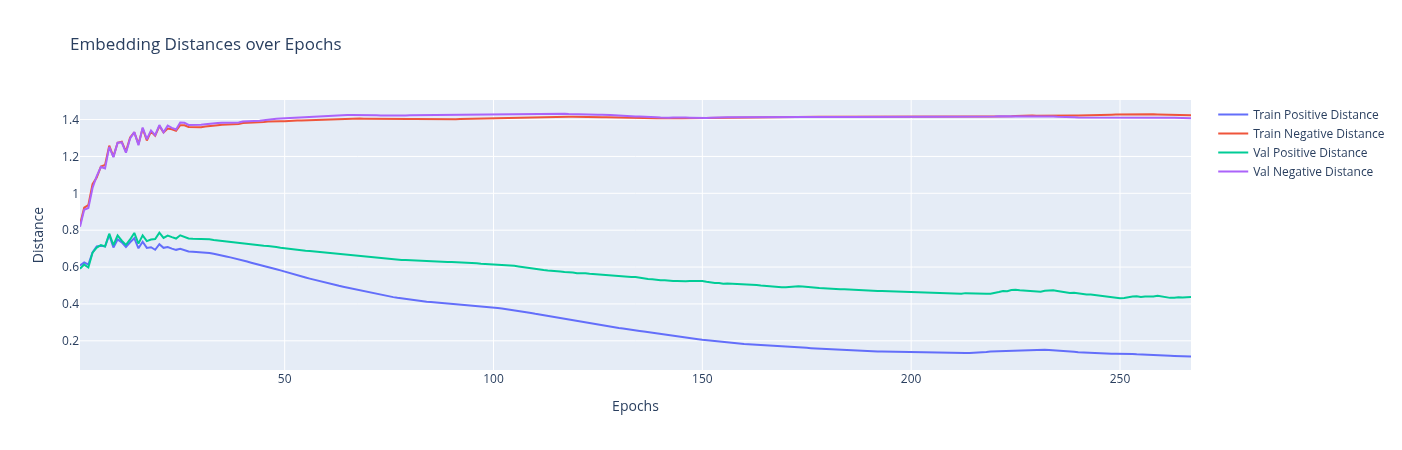
\includegraphics[width=0.6\textwidth]{figures/gloss-recognition/pos-neg-distances.png}
  \caption{Ewolucja średnich odległości par pozytywnych i negatywnych
  w trakcie treningu.}
  \label{fig:pos-neg-distances}
\end{figure}

\subsubsection{Podsumowanie}

Przedstawiliśmy system rozpoznawania izolowanego języka migowego oparty na
wyszukiwaniu dla zadania video-to-gloss. Począwszy od surowego obrazu wideo,
potok ekstrakcji oparty na MediaPipe generuje sekwencje szkieletowych punktów
charakterystycznych dla poszczególnych klatek, które są następnie poddawane
przetwarzaniu wstępnemu obejmującemu sprawdzanie aktywności dłoni,
interpolację czasową, usuwanie klatek statycznych, wygładzanie filtrem
Savitzky'ego-Golaya, normalizację przestrzenną oraz ponowne próbkowanie do
stałej długości 60 klatek. Wstępnie przetworzone sekwencje są przenoszone
do przestrzeni cech o wyższym wymiarze za pomocą warstwy projekcji
rozkładanej w czasie, a następnie przekazywane do enkodera czasowego,
porównywanego w pięciu wariantach. Enkoder Transformer konsekwentnie
przewyższa wszystkie warianty rekurencyjne w większości ocenianych metryk
i zostaje wybrany jako podstawa dalszej analizy. Enkoder jest trenowany
z wykorzystaniem złożonego celu łączącego funkcję straty Multi-Similarity
z regularyzacyjnym składnikiem rekonstrukcji ($\gamma=0.25$), tworząc
geometrycznie uporządkowaną przestrzeń osadzeń, w której tożsamość glosy
jest odzwierciedlona przez przynależność do skupiska, a klasyfikator
$k$ najbliższych sąsiadów generuje ostateczne przewidywanie glosy.
Oceniany na podzbiorze 32 glos zbioru ASL Citizen system osiąga czułość
przekraczającą 0.75 dla wszystkich klas, przy czym znaczna liczba glos
osiąga idealną czułość. Głównym ograniczeniem zidentyfikowanym we wszystkich
wymiarach ewaluacji jest zmienność wewnątrzklasowa wynikająca z różnic
w sposobie wykonywania znaków przez poszczególne osoby migające, która
przejawia się zwiększonymi odległościami par pozytywnych i większym
rozproszeniem skupisk dla osób niewidzianych podczas treningu.

\subsubsection{Zaimplementowane i planowane rozszerzenia}

Kilka konkretnych kierunków rozwoju obecnego systemu odpowiada na określone
ograniczenia architektoniczne, metodologiczne oraz związane z zakresem zadania,
zidentyfikowane powyżej.

\textbf{Dynamic Time Warping (DTW) podczas wyszukiwania.} Oprócz
bezpośredniego wyszukiwania w przestrzeni embeddingów implementacja zawiera
opcjonalny etap DTW. FAISS najpierw wybiera zbiór kandydatów, po czym sekwencja
zapytania jest porównywana z sekwencjami kandydatów, a wybierana jest etykieta
o najmniejszej odległości DTW. DTW znajduje optymalne czasowe wyrównanie dwóch
sekwencji i jest odporne na przesunięcia czasowe oraz różnice prędkości -- oba
te czynniki są częstymi źródłami zmienności wewnątrzklasowej w produkcji języka
migowego. W przeciwieństwie do odległości euklidesowej, która wyrównuje
sekwencje według znaczników czasu niezależnie od wartości cech, DTW wyrównuje
je na podstawie zawartości. Mechanizm jest obecnie dostępny w benchmarku jako
drugi etap po wybraniu kandydatów przez FAISS; tryb rozpoznawania na żywo
wykorzystuje bezpośrednie wyszukiwanie FAISS oraz stabilizację predykcji
opisaną w Rozdziale~\ref{chap:sentence-level-translation}. Aby odległości
wyrównania wyznaczane przez DTW były znaczące, porównywane sekwencje muszą
znajdować się we wspólnej, geometrycznie spójnej przestrzeni. Jest to rolą
dekodera rekonstrukcyjnego wprowadzonego w tym rozdziale, który ogranicza
enkoder do generowania reprezentacji pozostających strukturalnie zakotwiczonych
w przestrzeni współrzędnych punktów charakterystycznych.

\textbf{Soft-DTW jako cel treningowy.} Standardowy DTW jest różniczkowalny
w sposób nieciągły i nie może być bezpośrednio stosowany w treningu
opartym na gradientach. Soft-DTW \cite{cuturi2017softdtw} rozwiązuje ten
problem poprzez zastąpienie twardego minimum po ścieżkach wyrównania
miękkim minimum po wszystkich kosztach wyrównania, wygładzanym za pomocą
parametru temperatury $\gamma_{DTW}$, który odzyskuje standardowy DTW
dla $\gamma_{DTW} \to 0$; zarówno wartość funkcji, jak i jej gradient
można obliczać w czasie kwadratowym za pomocą programowania dynamicznego,
dzięki czemu metoda jest możliwa do zastosowania jako funkcja straty
podczas treningu. Planujemy zbadać zastąpienie funkcji straty rekonstrukcji
MSE $\mathcal{L}_{rec}$ (Równanie~\ref{eq:mse-loss}) funkcją soft-DTW jako
celem dekodera, trenując dekoder -- a przez niego również enkoder --
z wykorzystaniem funkcji straty jawnie niezmiennej względem przesunięć
czasowych i zmian prędkości.

\textbf{FAISS dla wyszukiwania wektorowego.} Bazowy klasyfikator KNN wykonuje
dokładne wyszukiwanie najbliższych sąsiadów w całym zbiorze referencyjnych
osadzeń. W zaimplementowanym systemie etap wyszukiwania realizuje biblioteka
FAISS (Facebook AI Similarity Search) \cite{johnson2019faiss}. Indeks jest
budowany z embeddingów nagrań referencyjnych i zapisywany w pliku
\texttt{index.faiss}; odpowiadające im etykiety oraz mapowanie identyfikatorów
na nazwy glos są przechowywane w pliku \texttt{index\_labels.npz}.

Obecna implementacja używa indeksu \texttt{IndexFlatIP}, czyli dokładnego
wyszukiwania według iloczynu skalarnego. Przed dodaniem do indeksu embeddingi
referencyjne są normalizowane normą L2; identyczna normalizacja jest wykonywana
dla embeddingu zapytania. W tych warunkach ranking według iloczynu skalarnego
jest równoważny rankingowi według podobieństwa cosinusowego.

Podczas wnioskowania system pobiera zbiór kandydatów większy niż pojedynczy
najbliższy sąsiad. Predykcją jest etykieta najlepszego wektora referencyjnego,
a dodatkowo obliczane są podobieństwo \emph{score} oraz margines
\emph{margin}. Margines oznacza różnicę między wynikiem najlepszego kandydata
a wynikiem najwyżej sklasyfikowanego kandydata należącego do innej klasy.
Wartości te są wykorzystywane w trybie ciągłego rozpoznawania do odrzucania
niepewnych predykcji.

\textbf{Sieci splotowe grafów dla kodowania przestrzennego.} Obecny potok
przetwarzania wstępnego spłaszcza zestawy punktów charakterystycznych
dla poszczególnych klatek do nieustrukturyzowanych wektorów, usuwając
topologiczną strukturę grafu szkieletu (zob. Sekcja~\ref{sec:video-to-gloss-methods}
i \cite{correia2019stgcn}). Sieci Graph Convolutional Networks stanowią
zasadniczą alternatywę, kodując szkielet punktów charakterystycznych jako
graf z wcześniej zdefiniowaną macierzą sąsiedztwa odzwierciedlającą
połączenia anatomiczne i propagując informację wzdłuż krawędzi szkieletu
w celu uzyskania osadzeń poszczególnych węzłów jawnie uwzględniających
strukturę ich sąsiedztwa. Planujemy zbadać enkodery GCN działające na
poziomie pojedynczej klatki jako zamiennik warstwy liniowej rozłożonej
w czasie.

\textbf{Quaternion LSTM dla kodowania czasowego uwzględniającego rotację.}
Trójwymiarowe współrzędne punktów charakterystycznych opisują położenia
stawów, które z natury mają charakter rotacyjny: ruch stawu dłoni lub
palca jest zasadniczo rotacją w $SO(3)$, a nie translacją w $\mathbb{R}^3$.
Standardowe LSTM o wartościach rzeczywistych traktują te współrzędne jako
niezależne cechy skalarne i nie posiadają wbudowanego założenia dotyczącego
struktury rotacyjnej. Quaternion LSTM operuje w algebrze kwaternionów
$\mathbb{H}$, reprezentując rotacje za pomocą kwaternionów jednostkowych
i wykonując operacje bramkowania z wykorzystaniem iloczynu Hamiltona,
co nadaje sieci jawny priorytet strukturalny dotyczący transformacji
rotacyjnych. Planujemy ocenić enkoder czasowy oparty na quaternion-LSTM
jako alternatywę dla standardowego LSTM.

\textbf{Ciągłe tłumaczenie wielu gestów za pomocą CTC.} Obecny system
obsługuje wyłącznie rozpoznawanie izolowane: każda sekwencja wejściowa
odpowiada pojedynczej, wstępnie wysegmentowanej glosie. Rozszerzenie
w kierunku ciągłych, niesegmentowanych sekwencji migania -- w których
granice pomiędzy glosami są nieznane i muszą być wyznaczane jednocześnie
z tożsamością glosy -- jest przedmiotem Rozdziału~\ref{chap:sentence-level-translation}.
